\chapter{O Framework ETL4NoSQL}
% ---
Neste capítulo são apresentados os conceitos do \textit{framework} ETL4NoSQL, que consiste numa plataforma de \textit{software} para desenvolvimento de aplicações de ETL, mais especificamente uma ferramenta que auxilia a construção de processos de ETL buscando apoiar a modelagem, reutilização e desempenho dos processos. 

O ETL4NoSQL oferece um ambiente com componentes integrados para modelar processos de ETL e implementar funcionalidades utilizando uma linguagem de programação independente de uma GUI (\emph{Graphical User Interface} - Interface Gráfica do Usuário).


Para a especificação do \textit{framework} proposto neste trabalho, foram elencados os requisitos de \textit{software} utilizando a abordagem de desenvolvimento baseado em componentes, fundamentada no estudo de \cite{cheesman:2001}. Neste estudo, temos a separação entre a modelagem do domínio e da especificação. A modelagem de domínio consiste na definição dos casos de uso, do modelo conceitual e do modelo comportamental. Já a modelagem de especificação é segmentada em três partes, a parte de identificação de componentes, de interação entre os componentes e a especificação de componentes.  

%definidas as estruturas de dados dos ambientes de origem, destino e da área de processamento de dados e suas respectivas linguagens de manipulação de dados, e também, as principais funcionalidades dos sistemas de ETL, chamados mecanismos de ETL. Para realizar os processos de ETL, por meio de seus mecanismos, foi definido um controlador de operações que é capaz de se comunicar com os ambientes e os mecanismos de ETL. 

A seguir, são detalhados os requisitos de \textit{software}, os modelos de domínio, os modelos de especificação, as especificações dos componentes, o ambiente de implementação e as interfaces de programação do ETL4NoSQL.

% a arquitetura do sistema e a estrutura dos componentes utilizados no desenvolvimento do framework.

\clearpage
% ---
\section{Requisitos de software do ETL4NoSQL}


Requisitos de \textit{software} são descrições de como o sistema deve se comportar, definidos durante as fases iniciais do desenvolvimento do sistema como uma especificação do que deveria ser implementado (\cite{sommerville:2013}). Os requisitos podem ser divididos em funcionais e não funcionais, onde o primeiro descreve o que o sistema deve fazer, ou seja, as transformações a serem realizadas nas entradas de um sistema, a fim de que se produzam saídas, já o outro expressa as características que este \textit{software} vai apresentar (\cite{sommerville:2013}). 

O ETL4NoSQL é um \textit{framework} que tem como principal objetivo auxiliar na criação de aplicações de ETL ao se utilizar principalmente BDs NoSQL. Um sistema de \textit{software} pode ter seus dados armazenados em BDs relacionais, que seguem o modelo entidade e relacionamento, ou não relacionais, no qual possui pouca definição de esquema, não seguem um modelo específico e são regularmente chamados de BDs NoSQL (\cite{fowler:2013}). Os BDs NoSQL possuem quatro paradigmas frequentemente utilizados: Chave-Valor, Família de Colunas, Documentos e Grafo (\cite{fowler:2013}).

Os SGBDs relacionais utilizam uma linguagem de gerenciamento de dados padrão conhecida por SQL (Structure Query Language) (\cite{fowler:2013}), porém os SGBDs NoSQL não possuem uma linguagem em comum, como os SGBDs relacionais, cada SGBD NoSQL possui sua própria linguagem de gerenciamento de dados (\cite{fowler:2013}). Por isso, é essencial que haja um componente que seja capaz de fazer a leitura diretamente da fonte de dados e um componente que também possa carregar esses dados diretamente no seu destino, independente do seu tipo, saber se é um arquivo texto, um arquivo XML, SGBD relacional, SGBD NoSQL, entre outros. Um componente tem como uma de suas definições ser uma unidade de \textit{software} independente, que encapsula a sua implementação, e oferece serviços por meio de suas interfaces (\cite{itana:2005}).

Outra importante características ao especificar o uso do ETL4NoSQL são os processos de ETL, que possuem quatro etapas básicas: extração, limpeza/transformação e carga (\cite{kimball:2004}). O fluxo do processo de ETL inicia-se com a extração dos dados a partir de uma fonte de dados. A começar da extração, é possível que um componente passe os dados para uma APD (Área de Processamento de Dados), onde é permitido modelar os dados executando processos de limpeza e transformação por meio de mecanismos (mecanismos de ETL) como de junção, filtro, união, agregação e outros. E finalmente, os dados são carregados em uma estrutura de dados destino.

Dessa forma, o ETL4NoSQL possui um componente que permite a leitura dos dados de diversos SGBDs NoSQL, de arquivos textuais, além dos SGBDs relacionais. Outro componente que permite a execução dos mecanismos de ETL, bem como faz uso de componentes para o gerenciamento da execução dos mecanismos, a construção da sequência dos processos de ETL e a escolha do tipo de processamento. O ETL4NoSQL é composto também de um componente que permite carregar diretamente os dados no destino independente do seu tipo. No quadro \ref{requisitos} é apresentado os principais requisitos elencados do ETL4NoSQL. Definimos como importante as prioridades que são imprescindíveis para o desenvolvimento e funcionamento do \textit{framework}, e desejável as funcionalidades que aprimoram o uso do \textit{framework}, porém não interferem no seu principal objetivo.

\begin{table}[h]
	\centering
	\caption{Requisitos do ETL4NoSQL}
	\label{requisitos}
	\begin{tabular}{|p{3cm}| p{10cm}| p{2cm} |}
		\hline
		Funcionalidade & Requisito & Prioridade\\
		\hline
		Suporte à plataforma &  Ser independente de plataforma. & Importante\\
		\hline
		Suporte à fonte &  Ser capaz de ler diretamente da fonte de dados, independente do seu tipo, saber se é uma fonte SGBD relacional, arquivo de texto, XML ou NoSQL. & Importante\\
		\hline
		Suporte ao destino & Ser capaz de carregar diretamente os dado no destino, independente do  seu tipo, saber se o destino é SGBD relacional, arquivo de texto, XML ou NoSQL. & Importante\\
		\hline
		Suporte à modelagem & Apoiar na extração de dados de múltiplas fontes de dados, na limpeza dos dados, na transformação, agregação, reorganização e operações de carga. & Importante\\
		\hline
		Paralelismo &Apoiar as operações de vários segmentos e execução em paralelo, internamente. A ferramenta deve ser capaz de distribuir tarefas entre múltiplos servidores. & Importante\\
		\hline
		Programável &Apoiar o agendamento de tarefas de ETL e ter suporte para programação em linha de comandos usando programação externa. & Importante\\
		\hline
		Reutilização & Apoiar a reutilização dos componentes do \textit{framework} e da lógica das transformações para evitar a reescrita. & Importante\\
		\hline
		Apoio ao nível de \textit{debugging} & Apoiar o tempo de execução e a limpeza da lógica de transformação. O usuário deve ser capaz de ver os dados antes e depois da transformação. & Desejável\\
		\hline
		Implementação & Suportar a capacidade de agrupar os objetos ETL e implementá-los em ambiente de teste ou de produção, sem a intervenção de um administrador de ETL. & Desejável\\
		\hline
		Garantia de Qualidade & Ser capaz de estabelecer processos, métricas e avaliações que possibilitem e garantam a qualidade de \textit{software}. & Desejável\\
		\hline
		
		
	\end{tabular}
\end{table}


\section{Modelagem do Domínio de ETL4NoSQL}

A modelagem do domínio de ETL4NoSQL é apresentada a seguir por meio de seus três modelos: modelo conceitual, modelo de casos de uso e modelo de comportamento.

\subsection{Modelo Conceitual}

Os conceitos de entidades para aplicações de ETL identificadas para o ETL4NoSQL são: Fonte, Destino, Modelagem, Processamento, Operações, ProcessamentoDistribuído e ProcessamentoCentralizado. O modelo conceitual pode ser visualizado na figura \ref{modeloconceitual}.

\begin{figure}[h]
	\centering
	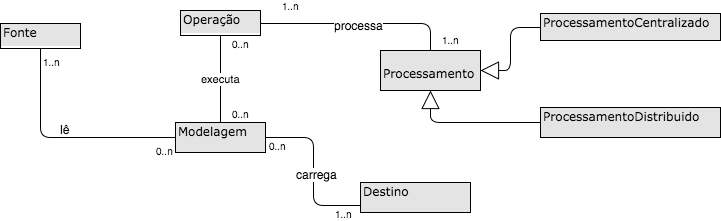
\includegraphics[scale=0.6]{fig/modeloconceitual.png}
	\caption{Modelo conceitual do ETL4NoSQL}
	\label{modeloconceitual}
\end{figure}

A entidade Modelagem faz a leitura de uma ou mais Fontes de dados, executa nenhuma ou muitas Operações. As Operações por sua vez são processadas por um ou mais Processamentos de forma a serem Processamentos Centralizados ou Processamentos Distribuídos. E por fim, a Modelagem carrega o resultado das Operações processadas à um ou mais Destinos.

Na subseção seguinte é apresentado o modelo de casos de uso do ETL4NoSQL.

\subsection{Modelo de Casos de Uso}

Os casos de uso expressam as funcionalidades fundamentais ao desenvolvimento e uso do ETL4NoSQL. Eles permitem ao programador a visão do que é imprescindível ao implementar e determinar as interfaces de sistema e operações do \textit{framework}. 

Um conjunto de casos de uso foram identificados tais como: Ler fonte de dados, Escrever no destino, Modelar dados, Executar operação e Processar operações. O quadro \ref{casosdeuso} mostra a descrição sucinta de cada caso de uso. 

Para finalizar a modelagem do domínio de ETL4NoSQL, a subseção seguinte apresenta o modelo comportamental do \textit{framework} proposto neste trabalho.



\begin{table}[h!]
	\centering
	\caption{Modelo de Casos de Uso do ETL4NoSQL}
	\label{casosdeuso}
	\begin{tabular}{|p{14cm}|}
		\hline
			\textbf{Nome:} Ler fonte de dados\\ 
			\textbf{Objetivo:} Fazer a leitura de qualquer tipo de dados a partir de uma fonte de dados.\\ 
			\textbf{Pré-condição:} os parâmetros para permissão de conexão com a fonte de dados devem estar disponíveis.\\ 
			\textbf{Ação:} ler (Fonte)\\ 
		\hline
			\textbf{Nome:} Escrever no destino\\ 
			\textbf{Objetivo:} Fazer a escrita de qualquer tipo de dado a partir do modelo processado pelo ETL4NoSQL em uma base  de dados de destino.\\ 
			\textbf{Pré-condição:} os parâmetros para permissão de conexão e escrita com o destino devem estar disponíveis.\\ 
			\textbf{Ação:} escrever (Destino)  \\ 
	\hline
			\textbf{Nome:} Modelar dados\\ 
			\textbf{Objetivo:} Permitir a modelagem dos dados por meio de mecanismos de junção, filtro, união, agregação e outros. \\
			 \textbf{Pré-condição:} os mecanismos de transformação e limpeza devem estar disponíveis para executar a modelagem.\\ 
			 \textbf{Ação:} modelar (Modelagem, Operação)\\ 
	 \hline
	 		\textbf{Nome:} Executar operação\\ 
	 		\textbf{Objetivo:} Armazenar, gerenciar e executar as operações criadas pela ação de modelar.\\
	 		\textbf{Pré-condição:} as operações devem ser criadas previamente pela ação de modelar.\\ 
	 		\textbf{Ação:} executar (Operação, Processamento)\\ 
	 \hline
	 	\textbf{Nome:} Processar operações\\ 
	 	\textbf{Objetivo:} Processar as operações armazenadas de forma centralizada ou distribuída.\\
	 	\textbf{Pré-condição:} as operações precisam estar disponíveis para o processamento.\\ 
	 	\textbf{Ação:} processar (Processamento, Operação)\\ 
	 \hline
	 
	\end{tabular}
\end{table}

\subsection{Modelo Comportamental}

Ao construir o modelo comportamental é possível identificar os conceitos com comportamentos mais relevantes para o negócio, bem como os estados e eventos que disparam as transições entre os estados (\cite{itana:2005}). Dessa forma, o diagrama de estados do ETL4NoSQL é apresentado na figura \ref{diagrama_estado}, nele podemos ver as transições de leitura da fonte de dados, validação e identificação dos dados, assim como o tratamento caso os dados não possam ser identificados. Subsequente a isso, podemos ver as transições do armazenamento dos dados para o processamento, a criação dos processos de ETL, a escolha da forma de processamento, execução das operações, e também o tratamento para as operações que não puderem ser executadas. Finalmente, a transição da carga dos dados pode ser feita na base de destino seguido da mensagem de tratamento, caso haja sucesso ou não na execução.

\begin{figure}[h!]
	\centering
	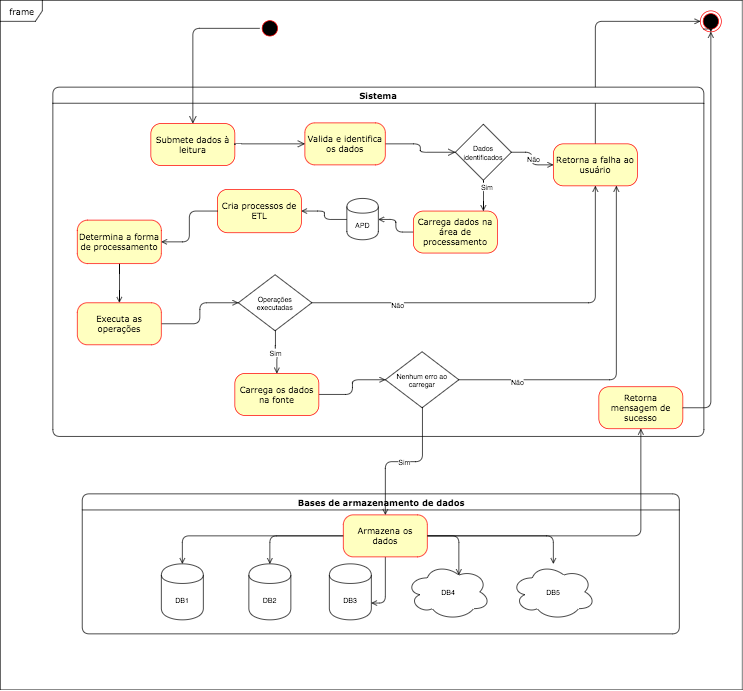
\includegraphics[scale=0.6]{fig/diagrama_estado.png}
	\caption{Diagrama de Estado do ETL4NoSQL}
	\label{diagrama_estado}
\end{figure}

\section{Modelagem da Especificação do ETL4NoSQL}

A modelagem de especificação visa definir, em um nível alto de abstração, os serviços oferecidos pelos componentes (\cite{itana:2005}). Dessa forma, é possível determinar a arquitetura e especificar os seus componentes. É importante dar ênfase a especificação das interfaces, pois isso contribui para uma clara separação entre os componentes, e também, para assegurar o princípio de encapsulamento de dados e comportamento (\cite{itana:2005}). \cite{cheesman:2001} divide a modelagem da especificação em três estágio, sendo assim, os estágios da modelagem de especificação do ETL4NoSQL são apresentados a seguir.


\subsection{Identificação de Componentes}
Seguindo o modelo de conceitos do negócio e do modelo de casos de uso foi possível identificar as interfaces para os componentes de negócio, as interfaces de sistema para os componentes de sistema e gerar a arquitetura de componentes inicial. As interfaces de negócio são reconhecidas por meio do modelo conceitual,  as interfaces de sistema e operações a partir dos casos de uso.

\subsection{Interfaces de Sistemas}

As interfaces de sistemas do ETL4NoSQL identificadas, por meio do modelo de casos de uso apresentado no quadro \ref{casosdeuso}, foram: IReadData, IWriteData, IModelData, IExeOp e IProcOp. Para especificar as interfaces foi utilizado OCL (Object Constraint Language) (\cite{warmer:1998}).
\\
\lstset{emph={%  
		context, pre, post%
	},emphstyle={\color{black}\bfseries\underbar}%
}%
\begin{lstlisting}[frame=single, language=Oberon-2, basicstyle=\small]
	context System :: IReadData (source : Fonte)	
	pre:	
	Fonte.allInstances@includes(Fonte) 
	Fonte.connection = estabelecido	
	Fonte.allInstances@includes(Fonte) 
	Fonte.connection = retorna mensagem de erro
	Fonte.allInstances@includes(Fonte) 
	Fonte.structureType =  reconhecido	
	Fonte.allInstances@includes(Fonte)
	Fonte.structureType = retorna mensagem de erro	
	
	post:
	Fonte. allInstances@includes 
	(f: Fonte | not Fonte.allInstances@pre@includes (f) and	
	Os atributos do objeto f foram inicializados)	
\end{lstlisting}

A partir da especificação foram identificadas as operações: Interface IReadData (Connection(connect) e structureType()).

\begin{lstlisting}[frame=single, language=Oberon-2, basicstyle=\small]
	context System :: IWriteData (load : Destino)
	pre:
	Destino.allInstances@includes(Destino) 
	Destino.connection = estabelecido
	Destino.allInstances@includes(Destino) 
	Destino.connection = retorna  erro
	Destino.allInstances@includes(Destino)
	Destino.structureType = reconhecido
	Destino.allInstances@includes(Destino)
	Destino.structureType = retorna  erro
	Destino.allInstances@includes(Destino) 
	Destino.structureType = permissao de escrita
	Destino.allInstances@includes(Destino)
	Destino.structureType = retorna  erro

	post:
	Fonte. allInstances@includes (d: Destino | not 
	Destino.allInstances@pre@includes (d) and
	Os atributos do objeto d foram inicializados)
\end{lstlisting}

As operações identificadas foram: Interface IWriteData (connection(connect), structureType() e allowWrite()).

\begin{lstlisting}[frame=single, language=Oberon-2, basicstyle=\small]
	context System :: IModelData (model : Modelagem; 
	source: Fonte; operation: Operacao)
	pre:
	Fonte.allInstances@includes(Fonte) 
	Fonte.connection = estabelecido and  
	Fonte.structureType = reconhecido	
	Fonte.allInstances@includes(Destino) 
	Fonte.connection = retorna  erro	
	Operacao.allInstances@includes(Operacao) 
	Operacao.mecanismo = existe	
	Operacao.allInstances@includes(Operacao) 
	Operacao.mecanismo = retorna erro	
	Modelagem.allInstances@includes(Modelagem) 
	Modelagem.operacao(dados)	
	post:	
	Modelagem. allInstances@includes (m: Modelagem | not 
	Destino.allInstances@pre@includes (m) and
	Os atributos do objeto m foram inicializados
	m foi ligado ao objeto f
	f.Fonte = Fonte
	m foi ligado ao objeto o
	o.Operacao = Operacao
	Todas as operacoes de modelagem foram criadas e 
	armazenadas em um APD)
\end{lstlisting}

As operações identificadas foram: Interface IModelData (readData(CodFonte) e createOp(CodOperação, data)).

\begin{lstlisting}[frame=single, language=Oberon-2, basicstyle=\small]
	context System :: IExeOp (model : Modelagem; operation: 
	Operacao, processing: Processamento)
	pre:
	Modelagem.allInstances@includes(Modelagem) 
	Modelagem.operacoes = existem 
	Operaaoo.allInstances@includes(Operacao) 
	Operacao.executa = retorna  erro	
	Operacao.allInstances@includes(Operacao) 
	Operacao.manage(operacoes)	
	post:
	Operacao. allInstances@includes (o: Operacao | not 
	Operacao.allInstances@pre@includes (o) and	
	Os atributos do objeto o foram inicializados
	o foi ligado ao objeto m
	m.Modelagem = Modelagem
	o foi ligado ao objeto p
	p.Processamento = Processamento
	Todas as operacoes escalonadas e estao pronta para 
	o processamento)

\end{lstlisting}

As operações identificadas foram: Interface IExeOp (modelOperation(CodModelagem) e operationManagement()).

\begin{lstlisting}[frame=single, language=Oberon-2, basicstyle=\small]
	context System :: IProcOp (operation: Operacao, 
	processing: Processamento)	
	pre:
	Operacao.allInstances@includes(Operacao) 
	Operacao.toExec = pronto	
	Processamento.allInstances@includes(Processamento) 
	Processamento.typeProc(tipoProcessamento)	
	post:		
	Processamento. allInstances@includes (m: Processamento 
	| not Destino.allInstances@pre@includes (p) and	
	Os atributos do objeto p foram inicializados
	p foi ligado ao objeto o
	o.Operacao = Operacao
	- Foi gerado o processamento das operacoes de acordo 
	com o tipo escolhido)

\end{lstlisting}

As operações identificadas foram: Interface IProcOp (process(CodOperação) e typeProc(tipoProcessamento)).

\subsection{Interfaces de Negócio}

Para definir as dependências no modelo, \cite{cheesman:2001} identificam o conceito de tipos principais, sendo estes tipos que possuem existência independente.
No ETL4NoSQL foi possível identificar quatro tipos principais: Fonte, Modelagem, Operação e Processamento. Para cada tipo principal foi possível definir uma interface de negócio, como é apresentado na figura \ref{modelo_negocio}.

\begin{figure}[h]
	\centering
	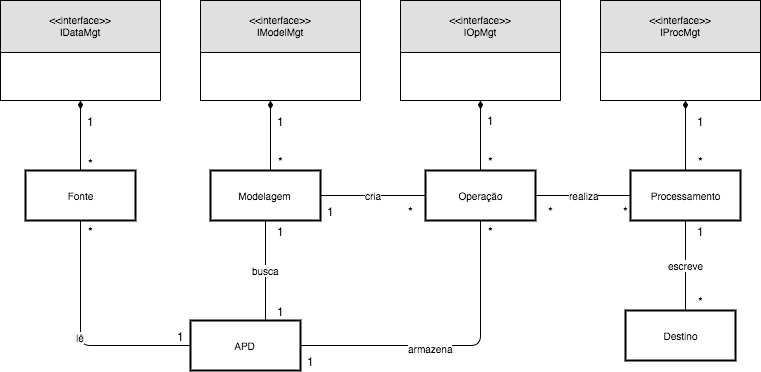
\includegraphics[scale=0.58]{fig/modelo_negocio.png}
	\caption{Definição de interfaces do modelo de negócio do ETL4NoSQL}
	\label{modelo_negocio}
\end{figure}

Na figura \ref{modelo_negocio} pudemos perceber a interação entre os componentes, porém essa interação será realizada por sua interface específica que será detalhada posteriormente na seção 3.4.

\subsection{Especificação da Arquitetura do Componente}

\cite{sommerville:2013}, define o projeto de arquitetura como um processo criativo em que se tenta organizar o sistema de acordo com os requisitos funcionais e não funcionais. Um estilo de arquitetura é um padrão de organização de sistema (\cite{shaw:1996}, \cite{sommerville:2013}), como uma organização cliente-servidor ou uma arquitetura em camadas. Porém, a arquitetura não necessariamente utilizará apenas um estilo, a maioria dos sistemas de médio e grande porte utilizam vários estilos. Para \cite{shaw:1996}, há três questões a serem definidas na escolha do projeto de arquitetura, a primeira é a escolha da estrutura, cliente-servidor ou em camadas, que permita atender melhor aos requisitos. A segunda questão é a respeito da decomposição dos subsistemas em módulos ou em componentes. E por fim, deve-se tomar a decisão de sobre como a execução dos subsistemas é controlada. A descrição da arquitetura pode ser representada graficamente utilizando modelos informais e notações como a UML (Unified Modeling Language) (\cite{clements:2002}, \cite{sommerville:2013}). Para o ETL4NoSQL, cada componente foi associado à sua interface de negócio identificada e uma interface de gerenciamento foi separada das outras interfaces de negócio, como pode ser visto na figura \ref{arquitetura}.

\begin{figure}[h]
	\centering
	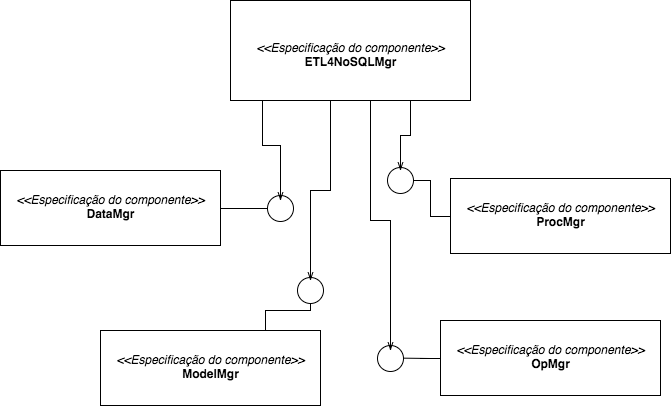
\includegraphics[scale=0.5]{fig/arquitetura_comp.png}
	\caption{Especificação da arquitetura do componente de ETL4NoSQL}
	\label{arquitetura}
\end{figure}

\section{Interação entre Componentes}

Esta etapa é detalhada, em termos de interações, utilizando diagramas de colaboração. Dessa forma, apresentamos os diagramas de colaboração para as interações do ETL4NoSQL na subseção a seguir.

\subsection{Operações da interface de negócio}

As operações de negócio são identificadas quando as interações forem analisadas para cada interface do sistema. Analisando as pré e pós-condições das operações de interface do sistema identificadas anteriormente foi possível detalhar usando diagramas de colaboração as interações necessárias para efetuar as operações do ETL4NoSQL. Os diagramas de colaboração de cada operação podem ser visto nas figuras de \ref{colaboracao1} até \ref{process}.

A conexão com a fonte de dados é estabelecida (figura \ref{colaboracao1}).

\begin{figure}[h!]
	\centering
	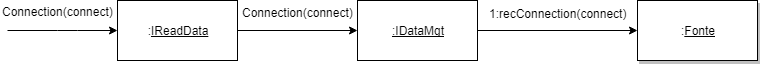
\includegraphics[scale=0.5]{fig/colaboracao1.png}
	\caption{Diagrama de colaboração para conectar à base de fonte de dados}
	\label{colaboracao1}
\end{figure}

A estrutura de dados da fonte é reconhecida (figura \ref{colaboracao2}).

\begin{figure}[h!]
	\centering
	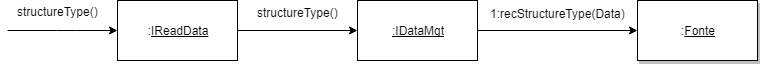
\includegraphics[scale=0.5]{fig/colaboracao2.png}
	\caption{Diagrama de colaboração para verificar a estrutura de dados}
	\label{colaboracao2}
\end{figure}

A escrita na base de dados destino é permitida (figura \ref{colaboracao3}).

\begin{figure}[h!]
	\centering
	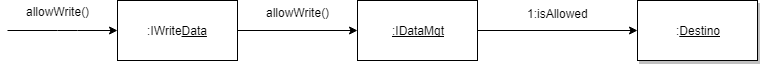
\includegraphics[scale=0.5]{fig/colaboracao3.png}
	\caption{Diagrama de colaboração para verificar se existe permissão de escrita na base de dados destino}
	\label{colaboracao3}
\end{figure}

A leitura dos dados da fonte é feita e armazenada na área de processamento de dados figura (\ref{readData}).

\begin{figure}[h!]
	\centering
	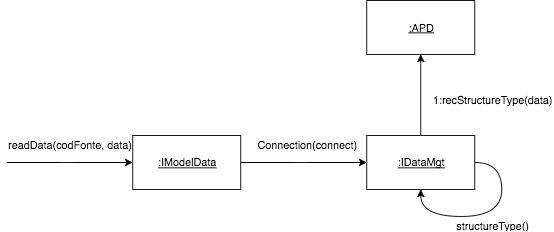
\includegraphics[scale=0.5]{fig/readData.png}
	\caption{Diagrama de colaboração para leitura dos dados da fonte}
	\label{readData}
\end{figure}

Após a leitura dos dados da fonte é possível a criação das operações por meio dos mecanismos existentes (figura \ref{createOp}).

\begin{figure}[h!]
	\centering
	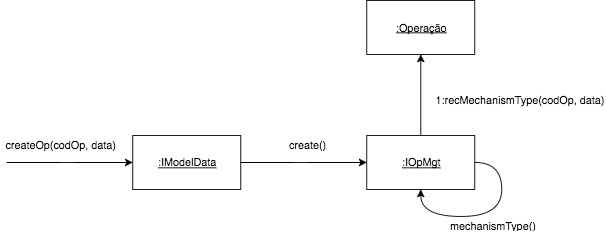
\includegraphics[scale=0.5]{fig/createOp.png}
	\caption{Diagrama de colaboração criação das operações de ETL}
	\label{createOp}
\end{figure}

Com as operações criadas, deve-se colocá-las em ordem de execução (figura \ref{modelOperation}).

\begin{figure}[h!]
	\centering
	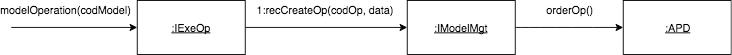
\includegraphics[scale=0.5]{fig/modelOperation.png}
	\caption{Diagrama de colaboração modelar as operações criadas}
	\label{modelOperation}
\end{figure}

É possível também que as operações sejam apagadas e alteradas (figura \ref{operationManagement}).

\begin{figure}[h!]
	\centering
	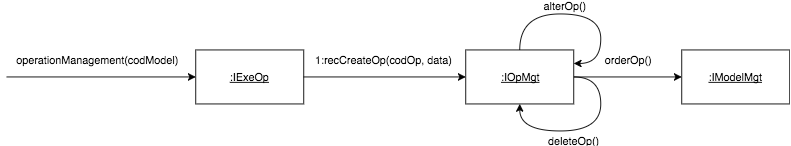
\includegraphics[scale=0.5]{fig/operationManagement.png}
	\caption{Diagrama de colaboração para gerenciar as operações}
	\label{operationManagement}
\end{figure}

Com as operações criadas é possível processá-las de forma a escolher o tipo de processamento (centralizado ou distribuído) (figura \ref{process}).

\begin{figure}[h!]
	\centering
	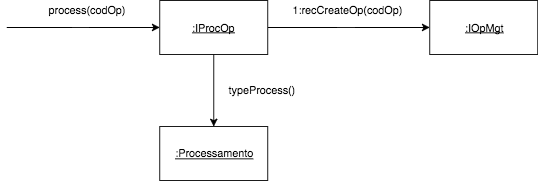
\includegraphics[scale=0.5]{fig/process.png}
	\caption{Diagrama de colaboração para processar as operações}
	\label{process}
\end{figure}

\section{Especificação de Componentes}

Posteriormente à definição das interfaces de negócio, é possível detalhá-las. Para cada interface, as operações são especificadas com suas assinaturas, pré e pós-condições.

\begin{lstlisting}[frame=single, language=Oberon-2, basicstyle=\small]

 context IDataMgt :: connection(connect):Fonte
	pre:
	- Existe um parametro de conexao "connect"
	- Existe uma fonte para ser conectada
	post:
	- A conexao com a fonte foi estabelecida ou nao
	- Recebe uma mensagem de conexao bem sucedida ou erro

 context IDataMgt :: strutuctureType():Fonte
	pre:
	- A conexao com a fonte foi bem sucedida
	post:
	- A estrutura de dados foi reconhecida ou nao
	- Retorna mensagem de sucesso ou erro
		
 context IDataMgt :: allowWrite():Destino
	pre:
	- A conexao com o destino foi bem sucedida
	post:
	- A base de dados destino permite escrita ou nao
	- Retorna mensagem de sucesso ou erro
	
 context IModelMgt :: readData(codFonte, data):APD
	pre:
	- A conexao com a fonte foi bem sucedida
	- A estrutura de dados foi reconhecida
	- Existe um parametro de busca "data" valido para 
		estrutura de dados reconhecida
	post:
	- A leitura dos dados foi realizada ou nao
	- Retorna os dados em uma APD ou uma mensagem de erro
		
 context IModelMgt :: createOp(codOp, data):Operacao
	pre:
	- Existe o mecanismo desejado para a criacao da operacao
	- Existe um parametro "data" com os dados a serem 
	usados na operacao
	post:
	- A operacao foi criada ou nao
	- Retorna o codOp ou uma mensagem de erro
		
 context IOpMgt :: modelOperation(codModel)
	pre:
	- Existem operacoes criadas na APD (codModel)
	post:
	- As operacoes sao ordenadas para execucao
		
 context IOpMgt :: operationManagement(codModel)
	pre:
	- Existem operacoes criadas na APD (codModel)
	post:
	- As operacoes foram alteradas, apagadas ou nao
	- Retorna mensagem de sucesso ou erro
	
 context IProcMgt :: process(codOp)
	pre:
	- Existe a operacao (codOp)
	- Foi escolhido o tipo de processamento 
	(centralizado ou distribuido)
	post:
	- A operacao foi processada ou nao
	- Retorna mensagem de sucesso ou erro
		
\end{lstlisting}

Depois das operações terem sido especificadas, o diagrama de especificação das interfaces foi criado e está representado na figura \ref{interfaces}. Essas especificações referem-se ao uso dos componentes. Elas representam o que o usuário precisa saber sobre os componentes.

\begin{figure}[h!]
	\centering
	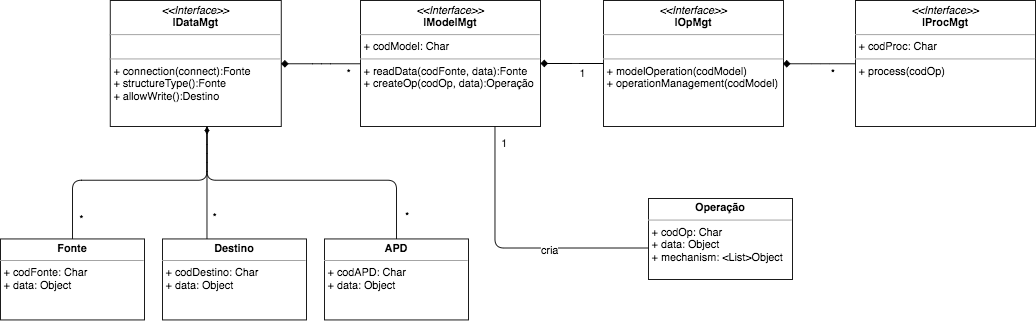
\includegraphics[scale=0.49]{fig/interfaces.png}
	\caption{Diagrama de especificação das interfaces de ETL4NoSQL}
	\label{interfaces}
\end{figure}

Nas próximas seções mostraremos o ambiente de implementação utilizado para desenvolver o ETL4NoSQL, bem como suas interfaces de programação.


\section{Ambiente de Implementação}

Para a implementação do ETL4NoSQL utilizamos a linguagem de programação Python, pois ela segue o paradigma de orientação à objetos que é adequado para a proposta desta pesquisa. Além disso, Python tem uma sintaxe de fácil aprendizado e pode ser usada em diversas áreas, como Web e computação gráfica. Ela é uma linguagem de alto nível interpretada e também é um software livre. Devido a natureza do \textit{framework} ser flexível, reusável e integrado faz com que a orientação à objetos torne-se um bom paradigma a ser aproveitado neste trabalho.

Assim, a implementação do \textit{framework} foi baseada nos princípios do \textit{design} orientado à objetos de inversão de controle, onde-se determina que os módulos de alto nível não devem ser dependentes de módulos de baixo nível, e sim, de abstrações, ou seja, os detalhes devem depender das abstrações. Esse princípio sugere que dois módulos não devem ser ligados diretamente, pois devem estar desacoplados com uma camada de abstração entre eles. Para suprir esse princípio, o ETL4NoSQL possui interfaces como o ETL4NoSQLMgr, IDataMgr, IModelMgr, IOpMgr e IProcMgr (figura \ref{arquitetura}). Elas utilizam dos mesmos comportamentos para as diversas variações, porém aplicados de acordo com a especificidade de cada um. Outro princípio importante utilizado é o da segregação de interfaces onde os usuários não devem ser forçados a depender de interfaces que não necessitam, elas devem ser enxutas com métodos específicos para cada interface. 

Na seção seguinte apresentaremos as interfaces de programação do ETL4NoSQL, como uma sugestão a ser utilizada para a implementação deste trabalho de dissertação.


\section{Interfaces de Programação}

O ETL4NoSQL possui cinco principais interfaces de programação (a arquitetura com as interfaces é apresentada na figura \ref{arquitetura}). O ETL4NoSQLMgr é a interface principal que interliga as demais interfaces, ela é a \textit{controller} (controlador) do \textit{framework}. Na figura \ref{etl4nosqlmgr} podemos ver a implementação da interface ETL4NoSQLMgr, nota-se que todas as outras quatro interfaces foram importadas nela (destaque 1 na figura \ref{etl4nosqlmgr}). Nesta interface, também é realizada a execução dos processos de leitura e escrita das bases de dados fonte, destino e área de processamento de dados (destaque 2 na figura \ref{etl4nosqlmgr}), cria a amostra dos dados a serem manipulados, as operações, realiza a execução das operações e as gerencia (destaque 3 na figura \ref{etl4nosqlmgr}).

\begin{figure}[h!]
	\centering
	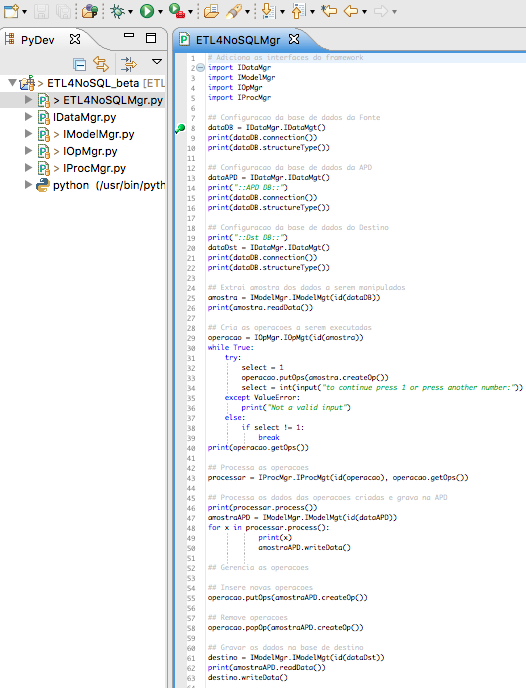
\includegraphics[scale=0.8]{fig/etl4nosqlmgr.png}
	\caption{Tela do IDE LiClipse com a implementação da interface ETL4NoSQLMgr}
	\label{etl4nosqlmgr}
\end{figure}

A interface IDataMgr pode ser vista na figura \ref{idatamgr}, ela é responsável pela conexão de todas as bases de dados, bem como determina o tipo de estrutura da base de dados, e também, informa se há permissão para escrita na base de dados desejada.

\begin{figure}[h!]
	\centering
	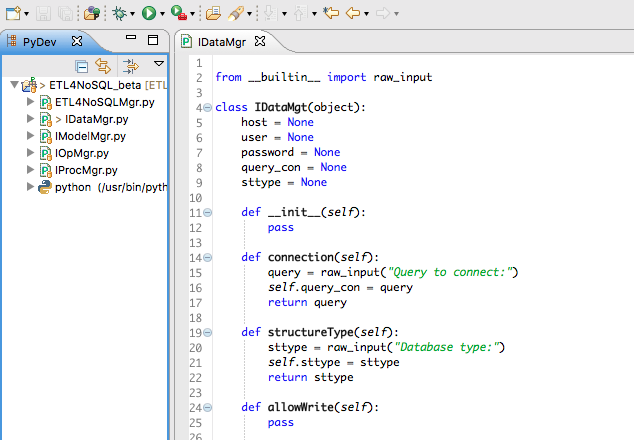
\includegraphics[scale=0.7]{fig/idatamgr.png}
	\caption{Tela do IDE LiClipse com a implementação da interface IDataMgr}
	\label{idatamgr}
\end{figure}

Na figura \ref{imodelmgr} é apresentada a interface IModelMgr, esta realiza a leitura dos dados da base armazenada pela interface IDataMgr e configurada pelo controlador ETL4NoSQLMgr. A interface IModelMgr também cria as operações de ETL e grava os dados na base de dados determinada no controlador. Note que nesta interface é possível criar novas operações de ETL, além da leitura e escrita, tornando o \textit{framework} flexível para cada aplicação. Ademais, após as operações serem criadas elas podem ser reutilizadas a qualquer momento facilitando o seu reuso.

\begin{figure}[h!]
	\centering
	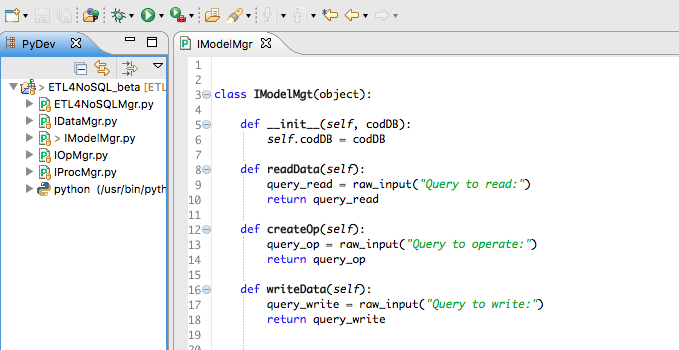
\includegraphics[scale=0.6]{fig/imodelmgr.png}
	\caption{Tela do IDE LiClipse com a implementação da interface IModelMgr}
	\label{imodelmgr}
\end{figure}

As operações criadas pela interface IModelMgr são listadas na interface IOpMgr (figura \ref{iopmgr}). Ela gerencia a inserção, alteração e remoção das operações, bem como ordena a sequência de operações a serem executadas conforme desejável pelo projetista de ETL.

\begin{figure}[h!]
	\centering
	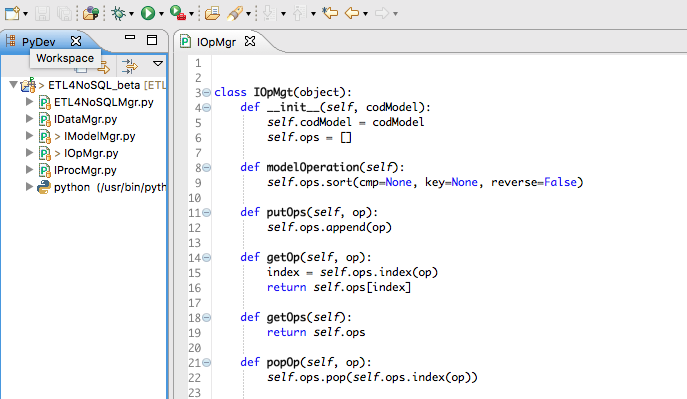
\includegraphics[scale=0.6]{fig/iopmgr.png}
	\caption{Tela do IDE LiClipse com a implementação da interface IOpMgr}
	\label{iopmgr}
\end{figure}

E finalmente, na figura \ref{iprocmgr}, é apresentada a interface IProcMgr. Esta interface é responsável pela execução das operações listadas pela IOpMgr. Na IProcMgr também é possível determinar e implementar o tipo de processamento das operações: distribuído, centralizado e paralelo. 

\begin{figure}[h!]
	\centering
	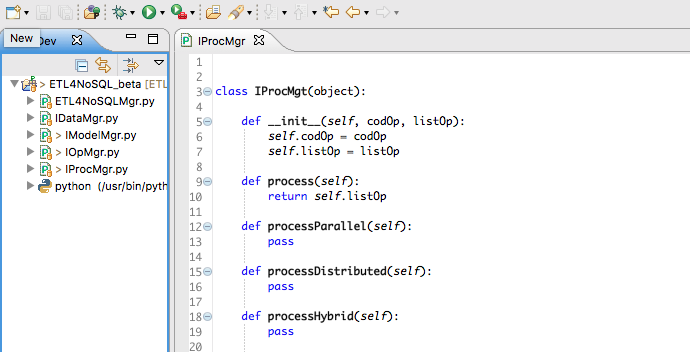
\includegraphics[scale=0.6]{fig/iprocmgr.png}
	\caption{Tela do IDE LiClipse com a implementação da interface IProcMgr}
	\label{iprocmgr}
\end{figure}

%De forma a detalhar a modelagem de especificação dos componentes deste trabalho, criamos um \textit{workflow} que é apresentado na figura \ref{modeloespecificacao} utilizando modelos informais e notações como a UML (\cite{clements:2002}).

%O modelo de processo do funcionamento da ferramenta ETL4NoSQL, baseado nas notações da UML 2.0 (\cite{clements:2002}), é representado na figura \ref{modeloprocesso}. Esse modelo descreve o processamento dos dados nas atividades de identificação dos dados, obtenção das informações para a importação e o mapeamento dos dados para os esquemas desejados, e também, a atividade dos processos de ETL para por fim dar carga dos dados em DWs, repositórios analíticos ou em arquivos XML.


% fluxo de processos da ferramenta ETL4NoSQL é o diagrama de atividades, que de acordo com a UML 2.0 tem como objetivo mostrar o fluxo de atividades em um único processo. O diagrama mostra como um atividade depende uma da outra. Na figura \ref{diagramaatividades} o diagrama mostra a interação dos componentes ao executar um processo de ETL, onde o estágio inicial é a importação dos dados seguido pelo mapeamento, após a obtenção dos dados necessários é possível a execução dos diversos processos de ETL em uma área de processamento para finalmente os dados serem exportados para base de destino.
%% utilizar diagrama de fluxo de dados para descrever os requisitos do sistema e diagrama de interações


%%construir um diagrama de atividades da execução de um processo de ETL



\section{Considerações Finais}

Este capítulo descreveu o \textit{framework} ETL4NoSQL. Para isso, foram apresentados os seus requisitos de desenvolvimento e exposta a sua modelagem do domínio por meio de seu modelo conceitual, de casos de uso e comportamental. Foram demonstradas a modelagem da especificação e identificado os componentes, as interfaces de sistemas e de negócio do \textit{framework} proposto, além da especificação da arquitetura dos componentes do ETL4NoSQL, bem como suas interações. Mostramos como solução para implementação do \textit{framework} um ambiente de implementação utilizando a linguagem orientada à objetos chamada Python, e também suas interfaces de programação.

O próximo capítulo apresentará o estudo experimental de \textit{software} que tem como objetivo definir se o ETL4NoSQL é adequado para desenvolver processos de ETL em BDs NoSQL e quais das suas funções são possíveis aprimorar.


%um estudo experimental de \textit{software} que tem por objetivo avaliar se o ETL4NoSQL é um \textit{framework} adequado para modelar e executar operações de ETL em BDs NoSQL.

